\section{非周期信号的傅里叶变换}

本节介绍非周期信号的傅里叶变换。
傅里叶变换是频域分析的重要方法,也是各种其他变换的基础。

本节要点:
\begin{itemize}
    \item 深入理解傅里叶变换及其物理意义;
    \item 理解傅里叶变换的量纲;
    \item 理解傅里叶变换的条件;
    \item 熟悉傅里叶变换的极坐标形式;
    \item 了解傅里叶级数和傅里叶变换的关系。
\end{itemize}

\begin{tcolorbox}
建议和《微积分》课程中的傅里叶积分对比着学习!
\end{tcolorbox}

%============================================================
\subsection{傅里叶变换的概念}

\begin{definition}[傅里叶变换]
若非周期信号$x\left( t \right) $满足:
\begin{itemize}
    \item 任一有限区域上满足狄利克雷收敛条件,
    \item 整个实数域绝对可积,即$\int_{-\infty}^{+\infty}{\left| x\left( t \right) \right|dt}$收敛,
\end{itemize}
则有:
\[
x\left( t \right) =\frac{1}{2\pi}\int_{-\infty}^{+\infty}{\left[ \int_{-\infty}^{+\infty}{x\left( t \right) e^{-i\omega t}dt} \right] e^{i\omega t}d\omega}
\]
对$x\left( t \right) $所有的连续点成立,称为{\bf $x\left( t \right) $的傅里叶积分},在间断点$t_0$处,可以用$\frac{1}{2}\left[ x\left( {t_0}^+ \right) +x\left( {t_0}^- \right) \right] $代替。
同时称$\int_{-\infty}^{+\infty}{x\left( t \right) e^{-i\omega t}dt}$为{\bf 信号$x\left( t \right) $的傅里叶变换}(Fourier transform,FT),记为$X\left( \omega \right) $即:
\[
X\left( \omega \right) =\int_{-\infty}^{+\infty}{x\left( t \right) e^{-i\omega t}dt}
\]
相应地称
\[
x\left( t \right) =\frac{1}{2\pi}\int_{-\infty}^{+\infty}{X\left( \omega \right) e^{i\omega t}d\omega}
\]
为{\bf 傅里叶逆变换}。
信号及其傅里叶变换形式通常记为:
\[
x\left( t \right) \overset{\mathscr{F}}{\leftrightarrow}X\left( \omega \right)
\]
\end{definition}

傅里叶变换是针对非周期信号而言的,所以没有基频这个概念,频率是一片连续的范围,与之相对的是周期信号的傅里叶级数的频率是无穷个离散值,可以想象成“连续谱”vs“线状谱”,傅里叶级数中的系数也从离散的$C_n$变成连续的$X\left( \omega \right) $。

如果信号在时域占满整个实数域$\mathbb{R} $,则对应傅里叶变换的频率在一个区间$\left( -\omega _0,+\omega _0 \right) $,相反,如果信号在时域是一个区间$\left( t_1,t_2 \right) $,则在频域将占满整个频率$\mathbb{R} $,即信号要么时域有限,要么频域有限,通常来讲,一般物理信号都是时域有限信号,所以是频域无限。

傅里叶变换和逆变换的对称性可知,只要信号能有傅里叶变换,则必有其傅里叶变换绝对可积,即$\int_{-\infty}^{+\infty}{\left| X\left( \omega \right) \right|d\omega}$收敛。

%============================================================
\subsection{傅里叶变换的量纲}

从定义式易得$X\left( \omega \right) $的量纲是信号的量纲乘以时间的量纲,或者说是信号的量纲除以频率的量纲$\mathrm{D}_x\cdot \mathrm{Hz}^{-1}$,这点是和傅里叶级数的区别。
{\bf $X\left( \omega \right) $的物理意义可以理解为单位频率的信号,或者说信号的频率密度。}
有些教材中会使用“信号分布在低频”这样的说法!

%============================================================
\subsection{傅里叶级数和傅里叶变换对比}

傅里叶级数和傅里叶变换的对比见下表:

\begin{table}[h]
\centering
% \caption{表头}
\begin{tabular}{ccc}
    \toprule
    & 傅里叶级数 & 傅里叶变换\\
    \midrule
    目标函数 & 周期函数 & 非周期函数\\
    展开 & $x\left( t \right) =\sum_{n=-\infty}^{+\infty}{\left( C_ne^{i\omega _nt} \right)}$ & $x\left( t \right) =\frac{1}{2\pi}\int_{-\infty}^{+\infty}{X\left( \omega \right) e^{i\omega t}d\omega}$\\
    角频 & 离散值,$\omega _n=n\omega _0=n\frac{2\pi}{T}$ & 连续值,$\omega \in \mathbb{R} $\\
    系数 & $C_n=\frac{1}{T}\int_{-\frac{T}{2}}^{\frac{T}{2}}{x\left( t \right) e^{-i\omega _nt}dt}$ & $X\left( \omega \right) =\int_{-\infty}^{+\infty}{x\left( t \right) e^{-i\omega t}dt}$\\
    \bottomrule
\end{tabular}
\end{table}

总之,对于周期信号的傅里叶级数,角频和系数的取值都是离散值,对于非周期信号的傅里叶变换,角频和系数的取值都是连续值。
这点可以类比为离散信号和连续信号。

%============================================================
\subsection{傅里叶变换的极坐标形式}

由于傅里叶变换有复指数项,所以结果一般是一个复数函数,可以变成极坐标形式:
\begin{align*}
X\left( \omega \right) &=\int_{-\infty}^{+\infty}{x\left( t \right) e^{-i\omega t}dt} \\
&=\int_{-\infty}^{+\infty}{x\left( t \right) \cos \left( \omega t \right) dt}+i\int_{-\infty}^{+\infty}{-x\left( t \right) \sin \left( \omega t \right) dt} \\
&=R\left( \omega \right) +iI\left( \omega \right)
\end{align*}
于是:
\begin{align*}
&\therefore \begin{cases}
	X\left( \omega \right) =\sqrt{R^2\left( \omega \right) +I^2\left( \omega \right)}\\
	\angle X\left( \omega \right) =\mathrm{arc}\tan \frac{I\left( \omega \right)}{R\left( \omega \right)}\\
\end{cases} \\
&\therefore X\left( \omega \right) =\left| X\left( \omega \right) \right|\cdot e^{i\angle X\left( \omega \right)}
\end{align*}
可以做类比:
\begin{itemize}
    \item $X\left( \omega \right) $:相当于傅里叶级数中的复指系数$C_n$;
    \item $\left| X\left( \omega \right) \right|$:相当于傅里叶级数中的幅度$A_n$;
    \item $\angle X\left( \omega \right) $:相当于傅里叶级数中的相位$\varphi _n$。
\end{itemize}

%============================================================
\subsection{广义傅里叶变换}

对于有些函数,如$x\left( t \right) =1,x\left( t \right) =\sin t$等,由于不满足狄利克雷条件,没有严格意义上的傅里叶变换,但可以通过单位冲激结合傅里叶变换的性质定义广义傅里叶变换。

单位冲激的傅里叶变换:
\begin{align*}
&\because \int_{-\infty}^{+\infty}{\delta \left( t \right) e^{i\omega t}dt}=\int_{-\infty}^{+\infty}{\delta \left( t \right) dt}=1 \\
&\therefore \delta \left( t \right) \leftrightarrow 1
\end{align*}
通过Duality,$x\left( t \right) =1$的广义傅里叶变换:
\[
1\leftrightarrow 2\pi \delta \left( \omega \right)
\]
以上只是一个例子,通过$\delta \left( t \right) $的傅里叶变换和傅里叶变换的性质,我们可以求得很多函数的广义傅里叶变换。

%============================================================
\subsection{傅里叶变换的性质}

{\bf 奇偶性}

如果$x\left( t \right) $是偶函数,则其傅里叶变换是实函数,如果$x\left( t \right) $是奇函数,则其傅里叶变换是纯虚函数,除此之外,一般傅里叶变换是复变函数。
\begin{align*}
&x\left( t \right) \text{ is even} \quad \Rightarrow \quad X\left( \omega \right) =\int_{-\infty}^{+\infty}{x\left( t \right) \cos \left( \omega t \right) dt} \\
&x\left( t \right) \text{ is odd} \quad \Rightarrow \quad X\left( \omega \right) =-i\int_{-\infty}^{+\infty}{x\left( t \right) \sin \left( \omega t \right) dt}
\end{align*}

{\bf 线性性}(由于积分的线性性,不证自明)
\[
ax\left( t \right) +by\left( t \right) \leftrightarrow aX\left( \omega \right) +bY\left( \omega \right)
\]

{\bf 时移性、频移性}(积分变量做一个变换即可证明)
\begin{align*}
&x\left( t-t_1 \right) \leftrightarrow X\left( \omega \right) e^{i\omega t_1} \\
&e^{i\omega t_1}x\left( t \right) \leftrightarrow X\left( \omega -\omega _1 \right)
\end{align*}

“时移性”表示信号在时域的延迟对傅里叶变换的结果是所有频率分量都慢了一个相位(即旋转),大小不变。
物理上讲,因为时间起点是人为设定的,所以信号的时移应具有FT的某种不变性。

{\bf 时展性}(积分变量做一个变换即可证明)
\begin{align*}
&x\left( at \right) \leftrightarrow \frac{1}{a}X\left( \frac{\omega}{a} \right) \\
&x\left( -t \right) \leftrightarrow -X\left( -\omega \right) =\bar{X}\left( \omega \right)
\end{align*}

“时展性”表示对时域的尺度变换对导致频域的尺度“相反地”变换。
这个容易理解,时域尺缩表示信号变化加快,自然频率尺扩,即高频分量增加。

{\bf 三角律}(频移性结合欧拉公式即可证明)
\begin{align*}
&x\left( t \right) \cos \omega _1t\leftrightarrow \frac{1}{2}\left[ X\left( \omega +\omega _1 \right) +X\left( \omega -\omega _1 \right) \right] \\
&x\left( t \right) \sin \omega _1t\leftrightarrow \frac{i}{2}\left[ X\left( \omega +\omega _1 \right) -X\left( \omega -\omega _1 \right) \right]
\end{align*}

{\bf 时域的微分和积分、频域的微分}
\begin{align*}
&\frac{d^nx\left( t \right)}{dt^n}\leftrightarrow \left( i\omega \right) ^n\cdot X\left( \omega \right) \\
&\int_{-\infty}^t{x\left( \tau \right) d\tau}\leftrightarrow \frac{1}{i\omega}\cdot X\left( \omega \right) \\
&\left( \frac{t}{i} \right) ^n\cdot x\left( t \right) \leftrightarrow \frac{d^nX\left( \omega \right)}{d\omega ^n}
\end{align*}

时域微分公式的前提是$\underset{t\rightarrow \pm \infty}{\lim} x\left( t \right) =0$。
时域积分通常来讲只有广义傅里叶变换,$\int_{-\infty}^t{x\left( \tau \right) d\tau}\leftrightarrow \frac{1}{i\omega}\cdot X\left( \omega \right) +\pi X\left( 0 \right) \delta \left( \omega \right) $。
特别地当时域信号没有直流分量时($X\left( 0 \right) =0$),才能得到上述公式。

{\bf 卷积性}
\begin{align*}
&x\left( t \right) \ast y\left( t \right) \leftrightarrow X\left( \omega \right) \cdot Y\left( \omega \right) \\
&x\left( t \right) \cdot y\left( t \right) \leftrightarrow \frac{1}{2\pi}\left[ X\left( \omega \right) \ast Y\left( \omega \right) \right]
\end{align*}

{\bf Parseval定理}
\begin{align*}
&\int_{-\infty}^{+\infty}{x\left( t \right) y\left( t \right) dt}=\frac{1}{2\pi}\int_{-\infty}^{+\infty}{\bar{X}\left( \omega \right) Y\left( \omega \right) d\omega} \\
&\int_{-\infty}^{+\infty}{x^2\left( t \right) dt}=\frac{1}{2\pi}\int_{-\infty}^{+\infty}{\left| X\left( \omega \right) \right|^2d\omega}
\end{align*}

{\bf Duality}
\[
X\left( t \right) \leftrightarrow 2\pi x\left( -\omega \right)
\]

%============================================================
\subsection{例}

\begin{example}
若有指数信号$x\left( t \right) =e^{-bt}u\left( t \right) $,求其傅里叶变换。
\end{example}

\begin{align*}
X\left( \omega \right) &=\int_{-\infty}^{+\infty}{x\left( t \right) e^{-i\omega t}dt}=\int_{-\infty}^{+\infty}{e^{-\left( b+i\omega \right) t}dt} \\
&=-\frac{1}{b+i\omega}\left[ \left. e^{-\left( b+i\omega \right) t} \right|_{0}^{+\infty} \right]
\end{align*}
当$b>0$时,有$\underset{t\rightarrow +\infty}{\lim} e^{-bt}=0$,则:
\[
X\left( \omega \right) =\frac{1}{b+i\omega}
\]
傅里叶变换是一个复数。
当$b\leqslant 0$时,$e^{-bt}$不收敛,信号不满足绝对可积条件,无傅里叶变换。

~

\begin{example}
若如下单方波信号,求其傅里叶变换,并分析脉宽和傅里叶变换之间的关系。
\[
p_{\tau}\left( t \right) =\begin{cases}
	1,t\in \left[ -\frac{\tau}{2},\frac{\tau}{2} \right]\\
	0,t\notin \left[ -\frac{\tau}{2},\frac{\tau}{2} \right]\\
\end{cases}
\]
\end{example}

先求傅里叶变换:
\begin{align*}
X\left( \omega \right) &=\int_{-\infty}^{+\infty}{x\left( t \right) e^{-i\omega t}dt}=\int_{-\frac{\tau}{2}}^{\frac{\tau}{2}}{e^{-i\omega t}dt} \\
&=\frac{1}{-i\omega}\left. e^{-i\omega t} \right|_{-\frac{\tau}{2}}^{\frac{\tau}{2}}=\frac{1}{-i\omega}\left( e^{-i\omega \frac{\tau}{2}}-e^{i\omega \frac{\tau}{2}} \right) \\
&=\frac{2}{\omega}\sin \frac{\omega \tau}{2}=\tau \frac{\sin \frac{\omega \tau}{2}}{\frac{\omega \tau}{2}}=\tau \mathrm{sinc}\frac{\omega \tau}{2\pi}
\end{align*}
由于信号是一个偶信号,傅里叶变换的结果是一个实数,它的相位永远只有0°和180°两个值。

以$\tau =0.5,\tau =1.5$两个脉宽的单方波信号为例,幅频图和相频图如下。

\begin{python}
w   = np.arange(-10*np.pi, 10*np.pi, 0.01)
tau = 0.5; X1 = tau * np.sinc(w*tau / 2 / np.pi)
tau = 1.5; X2 = tau * np.sinc(w*tau / 2 / np.pi)

plot_mag_phs(w, np.abs(X1), np.angle(X1, deg=True),
             axs[0][0], axs[1][0], title=r'$\tau =0.5$', ...)
plot_mag_phs(w, np.abs(X2), np.angle(X2, deg=True),
             axs[0][1], axs[1][1], title=r'$\tau =1.5$', ...)
\end{python}

\begin{figure}[h]
\centering
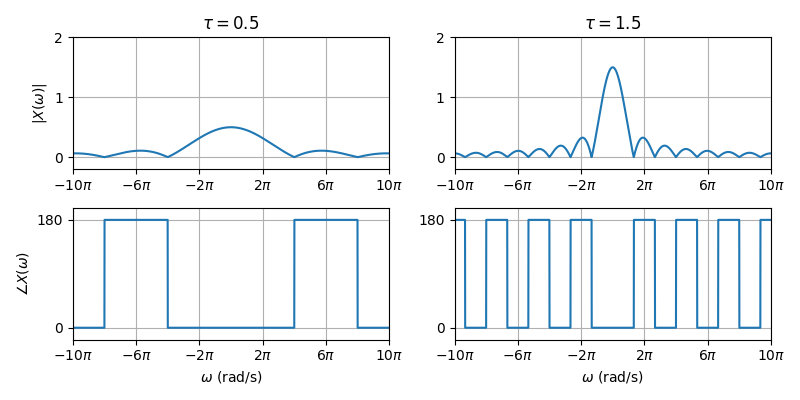
\includegraphics[height=5cm]{4.2.7-1.png}
\end{figure}

注意:
\begin{itemize}
    \item 所有图像的横坐标是角频$\omega $,单位是$\mathrm{rad}\cdot \mathrm{s}^{-1}$,为方便用弧度表示;
    \item $\underset{\tau \rightarrow 0}\lim p_{\tau}\left( t \right) =1,\underset{\tau \rightarrow 0}\lim X\left( \omega \right) =\delta \left( \omega \right) $。
\end{itemize}

